\documentclass{amsart}
\usepackage{../style}

\usepackage[margin = 1.25in]{geometry}

\captionsetup{justification = centering}

\title{Reedy Left Semi-Model Structure}
\author{Zack Dooley}
\date{}

\begin{document}
\maketitle

\section{Reedy Left Semi-Model Structure}

\begin{defn}
    A left semi-model structure on a bicomplete category consists of three classes of maps: $\cW,\cF,\cC$, subject to the axioms:
    \begin{enumerate}
        \item all three classes are closed under retracts and $\cW$ satisfies the 2-out-of-3 property;
        \item fibrations are preserved under pullbacks;
        \item cofibrations have the left lifting property with respect to trivial fibrations; and trivial cofibrations with a cofibrant source have the left lifting property with respect to fibrations;
        \item every map can be functorially factored into a cofibration followed by a trivial fibration; every map with a cofibrant source can also be functorially factored into a trivial cofibration followed by a fibration.
    \end{enumerate}
\end{defn}

\begin{lem}\label{lem:LA->LB cofib}
    Let $i:A\to B$ be a Reedy cofibration in $\cM^\cC$. The maps $A_\alpha\to B_\alpha$ and $L_\alpha A\to L_\alpha B$ are cofibrations in $\cM$ for all $\alpha\in\cC$.
\end{lem}
\begin{proof}
    This follows from \cite[Props. 15.3.9-10]{Hirshhorn} and the fact that cofibrations make up the left half of a weak factorization system in $\cM$.
\end{proof}

\begin{cor}\label{lem:cofib objs}
    Let $A$ be a Reedy cofibrant diagram in $\cM^\cC$. The objects $A_\alpha$ and $L_\alpha A$ are cofibrant in $\cM$ for all $\alpha\in\cC$.
\end{cor}

\begin{prop}\label{prop:pb's of fibs}
    Let $p:X\to Y$ be a Reedy fibration. The pullback of $p$ in $\cM^\cC$ is also a Reedy fibration.
\end{prop}
\begin{proof}
    Given the following pullback of diagrams,
    \[\begin{matrix}\begin{tikzpicture}
        \node (A) at (0,0) {$A\times_YX$};
        \node (X) at (2,0) {$X$};
        \node (B) at (0,-2) {$A$};
        \node (Y) at (2,-2) {$Y$};
        \draw[->] (A) to (B);
        \draw[->] (A) to (X);
        \draw[->>] (X) to (Y);
        \draw[->] (B) to (Y);
    \end{tikzpicture}\end{matrix}.\]
    We can now setup the following diagram,
    \[\begin{matrix}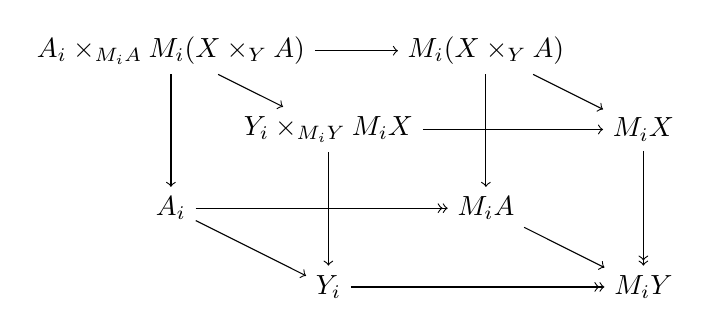
\begin{tikzpicture}
        \node (SX) at (-1,0) {$A_i\times_{M_iA}M_i(X\times_{Y}A)$};
        \node (SY) at (3,0) {$M_i(X\times_{Y}A)$};
        \node (X) at (-1,-2) {$A_i$};
        \node (Y) at (3,-2) {$M_iA$};
        \node (SA) at (1,-1) {$Y_i\times_{M_iY}M_iX$};
        \node (SB) at (5,-1) {$M_iX$};
        \node (A) at (1,-3) {$Y_i$};
        \node (B) at (5,-3) {$M_iY$};
        \draw[->] (X) to (A);
        \draw[->>] (X) to (Y);
        \draw[->>] (A) to (B);
        \draw[->] (Y) to (B);
        \draw[->] (SX) to (SA);
        \draw[->] (SX) to (SY);
        \draw[->] (SA) to (SB);
        \draw[->] (SY) to (SB);
        \draw[->] (SX) to (X);
        \draw[->] (SY) to (Y);
        \draw[->] (SA) to (A);
        \draw[->>] (SB) to (B);
    \end{tikzpicture}\end{matrix},\]
    where the front and back faces are pullbacks. Since the matching object is defined as a limit, we also know that $M_i(X\times_Y A)\cong M_iX\times_{M_iY}M_iA$, so the right face is a pullback as well. Using pullback pasting then, we can determine that the left face must be a pullback as well. Now looking at the induced maps, we can see
    \[\begin{matrix}\begin{tikzpicture}
        \node (XA) at (-2,0) {$X_i\times_{Y_i}A_i$};
        \node (X) at (2,0) {$X_i$};
        \node (AMXA) at (-2,-2) {$A_i\times_{M_iA}M_i(X\times_{Y}A)$};
        \node (YMX) at (2,-2) {$Y_i\times_{M_iY}M_iX$};
        \node (A) at (-2,-4) {$A_i$};
        \node (Y) at (2,-4) {$Y_i$};
        \node (MX) at (4,-2) {$M_iX$};
        \node (MY) at (4,-4) {$M_iY$};
        \draw[->] (XA) to (X);
        \draw[->] (XA) to (AMXA);
        \draw[->>] (X) to (YMX);
        \draw[->] (AMXA) to (YMX);
        \draw[->] (AMXA) to (A);
        \draw[->] (YMX) to (MX);
        \draw[->] (YMX) to (Y);
        \draw[->] (MX) to (MY);
        \draw[->] (A) to (Y);
        \draw[->] (Y) to (MY);
    \end{tikzpicture}\end{matrix}.\]
    We already know that the bottom two squares are pullbacks, so we get that the top square is as well, and thus the map $X_i\times_{Y_i}A_i\to A_i\times_{M_iA}M_i(X\times_{Y}A)$ is a fibration as desired. This shows that fibrations are stable under pullbacks.
\end{proof}

\begin{prop}\label{prop:factor c/tf}
    Let $\cM$ be a left semi-model category and $\cC$ a Reedy category. A map of diagrams $g:X\to Y$ in $\cM^\cC$ can be (functorially) factored as a Reedy cofibration followed by a Reedy trivial fibration.
\end{prop}
\begin{proof}
    We prove this by induction on degrees. First, for objects $\alpha$ of degree 0, we can use the factorization in $\cM$ to factor $g_\alpha$ as $X_\alpha\xrightarrow{i_\alpha}Z_\alpha\xrightarrow{h_\alpha}Y_\alpha$, where $i$ is a cofibration and $h$ is a trivial fibration.

    If we now assume that $g$ has been factored on all objects of degree less than $n$, and $\alpha$ is an object of degree $n$, then we have an induced map $X_\alpha\coprod_{L_\alpha X}L_\alpha Z\to Y_\alpha\times_{M_\alpha Y}M_\alpha Z$, which we can factor in $\cM$ to get
    $$ X_\alpha\sqcup_{L_\alpha X}L_\alpha Z\xrightarrow{i'}Z_\alpha\xrightarrow{h'} Y_\alpha\times_{M_\alpha Y}M_\alpha Z, $$
    where again $i'$ is a cofibration and $h'$ is a trivial fibration. This gives us our factorization of $g$, with $i$ a Reedy cofibration and $h$ a Reedy fibration. \cite[Lem 15.3.10]{Hirshhorn} states that since $h'$ is a trivial fibration (and thus has the right lifting property with respect to cofibrations), $h_\alpha$ also has the right lifting property with respect to cofibration, and is thus a trivial fibration (as the cofibrations and trivial fibrations make up a weak factorization system in $\cM$). This tells us that $h$ is a weak equivalence as well, so we have found our desired factorization.
\end{proof}

% Stronger Hypotheses
\begin{lem}\label{lem:semi-model struct}
    Suppose $\cM$ is a bicomplete category, equipped with
    \begin{enumerate}
        \item a class of maps $\cW$, including all identities, and closed under 2-out-of-6 and retracts;
        \item two weak factorization systems $(\cA,\cF)$ and $(\cC,\cT\cF)$;
        \item such that $\cT\cF=\cF\cap\cW$, and 
        \item when $A\in\cM$ is cofibrant, a map $i:A\to B$ is in $\cA$ if and only if it is in $\cC\cap\cW$.
    \end{enumerate}
    Then the classes $(\cW,\cC,\cF)$ form a left semi-model structure on $\cM$.
\end{lem}
\begin{proof}
    See \cite[Lem. 6.7]{KL}.
\end{proof}

\begin{lem}
    Suppose $\cM$ is a category which satisfies the hypotheses of \ref{lem:semi-model struct}. A pushout of a trivial cofibration with cofibrant source along a cofibration in $\cM$ is a trivial cofibration.
\end{lem}
\begin{proof}
    Consider the following pushout diagram,
    \[\begin{matrix}\begin{tikzpicture}
        \node (A) at (0,0) {$A$};
        \node (X) at (2,0) {$C$};
        \node (B) at (0,-2) {$B$};
        \node (Y) at (2,-2) {$P$};
        \draw[>->] (A) to node[left]{$\sim$} (B);
        \draw[>->] (A) to (X);
        \draw[->] (X) to (Y);
        \draw[->] (B) to (Y);
    \end{tikzpicture}\end{matrix}.\]
    Since left lifting properties are closed under pushouts, we know that the map $C\to P$ must have the left lifting property with respect to all fibrations. Because we have a weak factorization system $(\cA,\cF)$, this means that this map must be in the class $\cA$. Now, since $A$ is cofibrant and $A\to C$ is a cofibration, we get that $C\to P$ is a map in $\cA$ with cofibration source, so it must be a trivial cofibration.
\end{proof}

\begin{lem}\label{lem:LA->LB triv cofib}
    Suppose $\cM$ is a category which satisfies the hypotheses of \ref{lem:semi-model struct}. If the map $A\to B$ is a Reedy cofibration and a Reedy weak equivalence in $\cM^\cC$ and $A$ is Reedy cofibrant, then the maps $L_\alpha A\to L_\alpha B$ and $A_\alpha\coprod_{L_\alpha A}L_\alpha B\to B_\alpha$ are trivial cofibrations with cofibrant sources in $\cM$.
\end{lem}
\begin{proof}
    If we first assume that the map $L_\alpha A\to L_\alpha B$ is a trivial cofibration for some object $\alpha$, then the map $A_\alpha\to A_\alpha\coprod_{L_\alpha A}L_\alpha B$ is a pushout of a trivial cofibration with cofibrant source along a cofibration, so by the previous lemma it is a trivial cofibration. Since the map $A_\alpha\to B_\alpha$ is a weak equivalence by definition and it can be factored as $A_\alpha\to A_\alpha\coprod_{L_\alpha A}L_\alpha B\to B_\alpha$, this tells us that the cofibration $A_\alpha\coprod_{L_\alpha A}L_\alpha B\to B_\alpha$ is actually a trivial cofibration. To see that $A_\alpha\coprod_{L_\alpha A}L_\alpha B$ is cofibrant, we note that $A_\alpha$ is cofibrant and the map $A_\alpha\to A_\alpha\coprod_{L_\alpha A}L_\alpha B$ is a cofibration.

    We will now show that $L_\alpha A\to L_\alpha B$ is a trivial cofibration by induction on the degree of $\alpha$. First, in degree 0, the latching objects are both initial, so the map is automatically a trivial cofibration. Now, assuming that $L_\beta A\to L_\beta B$ is a trivial cofibration for all $\beta$ of degree less than the degree of $\alpha$, the previous part of the proof along with our inductive hypothesis implies that the map $A_\beta\coprod_{L_\beta A}L_\beta B\to B_\beta$ is a trivial cofibration. With this, \cite[lem. 15.3.9]{Hirshhorn} implies that $L_\alpha A\to L_\alpha B$ has the left lifting property with respect to all fibrations, which means it is in the class $\cA$, but it also has a cofibrant source, so it is a trivial cofibration.
\end{proof}

\begin{prop}\label{prop:factor tc/f}
    Let $\cM$ be a category satisfying the hypotheses of \ref{lem:semi-model struct}, and $\cC$ a Reedy category. A map of diagrams $f:X\to Y$, with $X$ Reedy cofibrant, in $\cM^\cC$ can be (functorially) factored as a Reedy trivial cofibration followed by a Reedy fibration.
\end{prop}
\begin{proof}
    This proof proceeds similarly to the previous factorization result. First, for $\alpha$ of degree 0, we can factor the map $X_\alpha\to Y_\alpha$ in $\cM$ as a trivial cofibration followed by a fibration since $X_\alpha$ is cofibrant, this gives us our degree 0 objects in the factorization, $Z_\alpha$. If we now assume we have factored $f$ on all objects of degree less than $\alpha$, we get an induced map $X_\alpha\coprod_{L_\alpha X}L_\alpha Z\to Y_\alpha\times_{M_\alpha Y}M_\alpha Z$, which we can apply factorization in $\cM$ again since \ref{lem:LA->LB triv cofib} tells us that the source is cofibrant. This gives us our factorization into a cofibration and a fibration, all that remains is to show that the map $X_\alpha\to Z_\alpha$ is a weak equivalence, but this follows from the fact that it can be factored as $X_\alpha\to X_\alpha\coprod_{L_\alpha X}L_\alpha Z\to Z_\alpha$, where the second map is a trivial cofibration by our factorization in $\cM$, and the first map is a trivial cofibration as a pushout of a trivial cofibration with cofibrant source along a cofibration. This completes our factorization.
\end{proof}

% Reedy left semi-model structure
\begin{thm}
    Let $\cM$ be a category satisfying the hypotheses of \ref{lem:semi-model struct}, and $\cC$ a Reedy category. The category $\cM^\cC$ comes equipped with a left semi-model structure where weak equivalences are component-wise, and (co)fibrations are Reedy (co)fibrations.
\end{thm}
\begin{proof}
    First, we know that $\cM^\cC$ is bicomplete as (co)limits are computed pointwise. Additionally, since weak equivalences are component-wise, they satisfy 2-out-of-3 and are closed under retracts. The (co)fibrations are also closed under retracts, as if $g:W\to Z$ is a retract of $h:X\to Y$, then the relative matching/latching maps of $g$ are retracts of the relative matching/latching maps of $h$.

    To show lifting of trivial cofibrations with cofibrant source, we construct the following diagram,
    \[\begin{matrix}\begin{tikzpicture}
        \node (A) at (0,0) {$A$};
        \node (X) at (2,0) {$X$};
        \node (B) at (0,-2) {$B$};
        \node (Y) at (2,-2) {$Y$};
        \draw[>->] (A) to node[left]{$\sim$} (B);
        \draw[->] (A) to (X);
        \draw[->>] (X) to (Y);
        \draw[->] (B) to (Y);
    \end{tikzpicture}\end{matrix}.\]
    We construct the lift inductively on the degree of objects. First, for $\alpha$ of degree 0, we get the following diagram,
    \[\begin{matrix}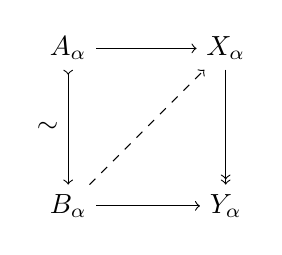
\begin{tikzpicture}
        \node (A) at (0,0) {$A_\alpha$};
        \node (X) at (2,0) {$X_\alpha$};
        \node (B) at (0,-2) {$B_\alpha$};
        \node (Y) at (2,-2) {$Y_\alpha$};
        \draw[>->] (A) to node[left]{$\sim$} (B);
        \draw[->] (A) to (X);
        \draw[->>] (X) to (Y);
        \draw[->] (B) to (Y);
        \draw[->, dashed] (B) to (X);
    \end{tikzpicture}\end{matrix},\]
    where the maps $A_\alpha\to B_\alpha$ and $X_\alpha\to Y_\alpha$ are a trivial cofibration and fibration, respectively, by the definition of Reedy (co)fibrations (noting that in degree 0, the latching objects are all initial and the matching objects are all terminal). The lift is then constructed using the lifting properties in $\cM$, noting that $A_\alpha$ is cofibrant by \ref{lem:cofib objs}. For the inductive step, all that is necessary is to construct a lift in the following diagram by \cite[15.2.11]{Hirshhorn},
    \[\begin{matrix}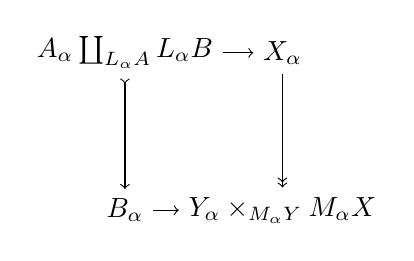
\begin{tikzpicture}
        \node (A) at (0,0) {$A_\alpha\coprod_{L_\alpha A}L_\alpha B$};
        \node (X) at (2,0) {$X_\alpha$};
        \node (B) at (0,-2) {$B_\alpha$};
        \node (Y) at (2,-2) {$Y_\alpha\times_{M_\alpha Y}M_\alpha X$};
        \draw[>->] (A) to (B);
        \draw[->] (A) to (X);
        \draw[->>] (X) to (Y);
        \draw[->] (B) to (Y);
    \end{tikzpicture}\end{matrix}.\]
    To get the requisite lift, we need to know that $A_\alpha\coprod_{L_\alpha A}B_\alpha$ is cofibrant in $\cM$ and that left map is a trivial cofibration in $\cM$, but this is given by \ref{lem:LA->LB triv cofib}.

    For lifting cofibrations against trivial fibrations consider the following diagram,
    \[\begin{matrix}\begin{tikzpicture}
        \node (A) at (0,0) {$A$};
        \node (X) at (2,0) {$X$};
        \node (B) at (0,-2) {$B$};
        \node (Y) at (2,-2) {$Y$};
        \draw[>->] (A) to (B);
        \draw[->] (A) to (X);
        \draw[->>] (X) to node[right]{$\sim$} (Y);
        \draw[->] (B) to (Y);
    \end{tikzpicture}\end{matrix}.\]
    The proof proceeds identically to the proof for the regular Reedy model structure. As before, we prove this by induction on the degree of $\alpha$, and in degree 0, we immediately get our lift by the definition of Reedy (co)fibrations. For the inductive step, all we need to show is that the map $X_\alpha\to Y_\alpha\times_{M_\alpha Y}M_\alpha X$ is a weak equivalence. To see this, we note that the map $X_\alpha\to Y_\alpha$ is a weak equivalence by definition, but this can be factored as $X_\alpha\to Y_\alpha\times_{M_\alpha Y}M_\alpha X\to Y_\alpha$, where the second map is a weak equivalence as a pullback of the map $M_\alpha X\to M_\alpha Y$ (This map is a trivial fibration by \cite[15.3.9]{Hirshhorn}, and trivial fibrations are closed under pullbacks as they make up the right half of a weak factorization system on $\cM$). Two-out-of-three then gives us that our desired map is a weak equivalence, so we can now finish the inductive step by constructing the lift in $\cM$.

    All that remains is our factorizations and to show that fibrations are preserved under pullbacks, but these were proven in \ref{prop:factor c/tf}, \ref{prop:factor tc/f}, and \ref{prop:pb's of fibs}, respectively. This gives us our desired left semi-model structure on $\cM^\cC$.
\end{proof}

\begin{cor}
    There exists a Reedy left semi-model structure on the category $\CxlCat^\Delta$.
\end{cor}
\begin{proof}
    For the verification of the hypotheses of \ref{lem:semi-model struct}, see \cite[\S 6]{KL}.
\end{proof}

\section{Simplicial Mapping Space}

\begin{defn}\cite[Def. 16.3.1]{Hirshhorn}
    Let $\cM$ be a left semi-model category.
    \begin{enumerate}
        \item If $\mathbf{X}$ is a cosimplicial object in $\cM$ and $K$ a simplicial set, then $\mathbf{X}\otimes K$ is defined as the colimit of the functor $F:\Delta\downarrow K\to\cM$ which sends an object $\Delta^n\to K$ of $\Delta\downarrow K$ to $\mathbf{X}^n$, and a map
        \[\begin{matrix}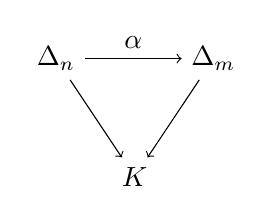
\begin{tikzpicture}
            \node (A) at (0,0) {$\Delta_n$};
            \node (X) at (2,0) {$\Delta_m$};
            \node (B) at (1,-1.5) {$K$};
            \draw[->] (A) to (B);
            \draw[->] (A) to node[above]{$\alpha$} (X);
            \draw[->] (X) to (B);
        \end{tikzpicture}\end{matrix},\]
        to the map $\alpha_*:\mathbf{X}^n\to\mathbf{X}^m$.
    \end{enumerate}
\end{defn}

\begin{notn}\cite[Not. 16.4.1]{Hirshhorn}
    Let $\cM$ be a left semi-model category.
    \begin{enumerate}
        \item If $\mathbf{X}$ is a cosimplicial object in $\cM$ and $Y$ is an object in $\cM$, then $\cM(\mathbf{X},Y)$ will denote the simplicial set defined by $\cM(\mathbf{X},Y)_n:=\cM(\mathbf{X}^n,Y)$ with face and degeneracy maps induced by the maps in $\mathbf{X}$.
    \end{enumerate}
\end{notn}

\begin{prop}
    Let $\cM$ be a left semi-model category.
    \begin{enumerate}
        \item If $i:\mathbf{A}\to\mathbf{B}$ is a map of cosimplicial objects in $\cM$, $p:X\to Y$ is a map in $\cM$, and $(K,L)$ is a pair of simplicial sets, then a lift exists in the following diagram on the left if and only if a lift exists in the following diagram on the right,
        \[\begin{matrix}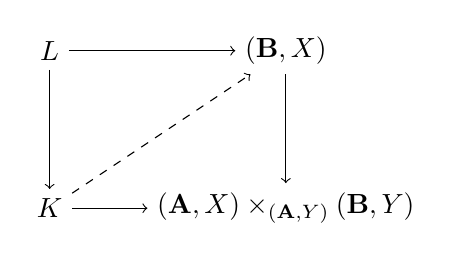
\begin{tikzpicture}
            \node (A) at (0,0) {$L$};
            \node (X) at (3,0) {$\cM(\mathbf{B},X)$};
            \node (B) at (0,-2) {$K$};
            \node (Y) at (3,-2) {$\cM(\mathbf{A},X)\times_{\cM(\mathbf{A},Y)}\cM(\mathbf{B},Y)$};
            \draw[->] (A) to (B);
            \draw[->] (A) to (X);
            \draw[->] (X) to (Y);
            \draw[->] (B) to (Y);
            \draw[->, dashed] (B) to (X);
        \end{tikzpicture}\end{matrix}\qquad\iff\qquad
        \begin{matrix}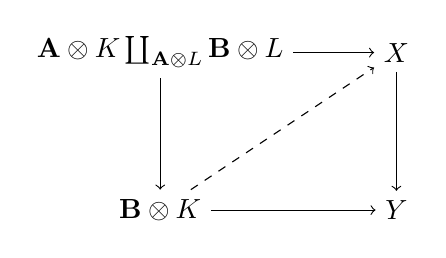
\begin{tikzpicture}
            \node (A) at (0,0) {$\mathbf{A}\otimes K\coprod_{\mathbf{A}\otimes L}\mathbf{B}\otimes L$};
            \node (X) at (3,0) {$X$};
            \node (B) at (0,-2) {$\mathbf{B}\otimes K$};
            \node (Y) at (3,-2) {$Y$};
            \draw[->] (A) to (B);
            \draw[->] (A) to (X);
            \draw[->] (X) to (Y);
            \draw[->] (B) to (Y);
            \draw[->, dashed] (B) to (X);
        \end{tikzpicture}\end{matrix}.\]
    \end{enumerate}
\end{prop}
\begin{proof}
    See \cite[Prop. 16.4.5]{Hirshhorn}. The same proof works with $\cM$ a left semi-model category as opposed to a full model category. 
\end{proof}

\begin{cor}
    Let $\mathbf{B}$ be a cosimplicial object in $\CxlCat$. The simplicial set $\CxlCat(\mathbf{B},\T)$ is a quasicategory if lifts exist in the following diagrams in $\CxlCat$ for all $n$ and all $0<k<n$,
    \[\begin{matrix}\begin{tikzpicture}
        \node (A) at (0,0) {$\mathbf{B}\otimes\Lambda_n^k$};
        \node (X) at (3,0) {$\T$};
        \node (B) at (0,-2) {$\mathbf{B}_n$};
        \draw[->] (A) to (B);
        \draw[->] (A) to (X);
        \draw[->, dashed] (B) to (X);
    \end{tikzpicture}\end{matrix}.\]
\end{cor}
\begin{proof}
    Take $i$ to be the map $0\to\mathbf{B}$, $p$ to be the map $\T\to1$, and $(K,L)=(\Lambda_n^k,\Delta_n)$.
\end{proof}

\newpage
\bibliographystyle{plain}
\bibliography{refs}

\end{document}